%%%%%%%%%%%%%%%%%%%%%%%%%%%%%%%%%%%%%%%%%
% Thin Sectioned Essay
% LaTeX Template
% Version 1.0 (3/8/13)
%
% This template has been downloaded from:
% http://www.LaTeXTemplates.com
%
% Original Author:
% Nicolas Diaz (nsdiaz@uc.cl) with extensive modifications by:
% Vel (vel@latextemplates.com)
%
% License:
% CC BY-NC-SA 3.0 (http://creativecommons.org/licenses/by-nc-sa/3.0/)
%
%%%%%%%%%%%%%%%%%%%%%%%%%%%%%%%%%%%%%%%%%

%----------------------------------------------------------------------------------------
%	PACKAGES AND OTHER DOCUMENT CONFIGURATIONS
%----------------------------------------------------------------------------------------

\documentclass[a4paper, 11pt]{article} % Font size (can be 10pt, 11pt or 12pt) and paper size (remove a4paper for US letter paper)

\usepackage[protrusion=true,expansion=true]{microtype} % Better typography
\usepackage{graphicx} % Required for including pictures
\usepackage{wrapfig} % Allows in-line images

\usepackage{mathpazo} % Use the Palatino font
\usepackage[T1]{fontenc} % Required for accented characters
\linespread{1.05} % Change line spacing here, Palatino benefits from a slight increase by default

\makeatletter
\renewcommand\@biblabel[1]{\textbf{#1.}} % Change the square brackets for each bibliography item from '[1]' to '1.'
\renewcommand{\@listI}{\itemsep=0pt} % Reduce the space between items in the itemize and enumerate environments and the bibliography

\renewcommand{\maketitle}{ % Customize the title - do not edit title and author name here, see the TITLE block below
\begin{flushright} % Right align
{\LARGE\@title} % Increase the font size of the title

\vspace{50pt} % Some vertical space between the title and author name

{\large\@author} % Author name
\\\@date % Date

\vspace{40pt} % Some vertical space between the author block and abstract
\end{flushright}
}

%----------------------------------------------------------------------------------------
%	TITLE
%----------------------------------------------------------------------------------------

\title{\textbf{Automatic Sleep Stages Classification}\\ % Title
} % Subtitle

\author{\textsc{} % Author
\\{\textit{}}} % Institution

\date{\today} % Date

%----------------------------------------------------------------------------------------

\begin{document}

\maketitle % Print the title section

%----------------------------------------------------------------------------------------
%	ABSTRACT AND KEYWORDS
%----------------------------------------------------------------------------------------

%\renewcommand{\abstractname}{Summary} % Uncomment to change the name of the abstract to something else

\begin{abstract}

\end{abstract}

\hspace*{3,6mm}\textit{Keywords:}   % Keywords

\vspace{30pt} % Some vertical space between the abstract and first section

%----------------------------------------------------------------------------------------
%	ESSAY BODY
%----------------------------------------------------------------------------------------
\section*{Literatre Review}
Oropesa et al.(1999) used Discrete Wavelet Transform (DWT) to extract energies of 7 EEG sub bands as features. They also defined 6 more features based on total energy and the relative energy of sub bands.The database which they used including only 2 EEG recording with 30 seconds long epochs. Artificial neural network (ANN) is used as a classification algorithm. They reached a $77.6\%$ of agreement. Zoubek et al.(2007) applied both DWT and fast fourier transform (FFT) to extract features. Their database consists of Four EEG
channels (C3-A2, P3-A2, C4-A1, and P4-A1) of 47 night sleep recordings of healthy adults which are divided into 20 second epochs. By using relative wavelet energy of 5 EEG sub bands, they obtained a total of $71\%$ of agreement. They included the features extracted from EOG and EMG channels to improve the accuracy about $80\%$.The classification approach of  Doroshenkov et al.(2007) was based on Hidden Markov Model (HMM). They used FFT to extract 4 features of sub bands.They used two EEG channels (Fpz-Cz and Pz-Oz) of 8 subjects from physionet online dataset. They achieved best result of accuracy for sllep stage 4 ($91.54\%$) and the worst one for sleep stage 1 ($4.84\%$).  Sinha (2008)classified three stages of sleep : awake (AWA), rapid eye movement (REM) and sleep spindles (SS). DWT method was used to extract features for 2 seconds epochs of 64 EEG data.  By applying ANN as a classifier, $95.55\%$ rate of accuracy was obtained. .Ebrahimi et al.(2008) used 7 EEG recordings from PhysioBank Database of Pz-Oz channel. DWT applied to extract features of 30 second epochs. They used energy, total energy, ratio of different energy values of 6 sub bands accordingly as well as mean of the absolute values of the coefficients and Standard deviation of the coefficients in each sub band. ANN is aplied as a classifier. The authors have achieved an accuracy rate of $93\%$ in the classification of 5 sleep stages.Gunes et al. (2009) proposed a novel data pre-processing called K-means clustering based feature weighting (KMCFW) and used Welch method to extract the features. They used three night sleep recording. They used C4.5 decision tree to classify 5 sleep stages. They achieved the success rate of $92.4\%$ by this method. Jo et el. (2010) designed the fuzzy classifier based
on the genetic algorithm (GA) for a single channel EEG signal (C3-A2). They used FFT for 30 second long epochs to obtain  relative power spectra of 5 EEG sub bands as features. Finally, they obtained the accuracy rate of $84.6\%$ in classifying of 4 sleep stages.  Tagluk et al.(2010) used a multi-layer neural network (NN) which simultaneously applied EEG, EMG and EOG. The dataset were obtained from 7 hours sleep recording of 21 subjects which including an EEG channel (C3–A2), EMG and EOG. They obtained the accuracy rate of $74.7\%$. Fraiwan et al. (2011) used 3 different methods of time-frequency Analysis to extract the features: Choi–Williams distribution (CWD), Continuous wavelet transform (CWT)and Hilbert–Huang Transform (HHT). By computing Renyi’s entropy of sub bands, 7 features were extracted. They used the recordings of a single EEG channel (C3-A1) for an entire night of sleep (6–8 h) of sixteen subjects. Random Forest (RF) is applied as a classifier. They obtained the accuracy rate of $83\%$, $78\%$ and $75\%$ for CWT, CWD and HHT , respectively. Ozsen et al. (2012) used ANN to classify 5 sleep stages. Five sleep recordings of EEG, EMG and EOG was used and the total accuracy rate of $90.93\%$ obtained. Koley and Dey (2012) extracted 39 features including Time domain, frequency domain and non-linear analysis (21 features finally selected). They used single channel EEG (C4-A1) recordings of 28 subjects (having sleep apnea) during one night sleep. They used support vector machine (SVM) as a classifier and achieved the accuracy rate of $91.1\%$. Liang et al (2012) applied a linear classifier to classify the features of multiscale entropy (MSE) and auto regressive (AR). They used the recordings of 20 healthy subjects of single EEG channel(C3-A2). They obtained the total accuracy rate of $85.38\%$.Hsu et al. (2013) applied FFT to extract energy features of sub bands and NN to classify sleep stages. The data set consisted of recordings from single EEG channel (Fpz-Cz)of 8 subjects during 24 hour of daily life (physionet online dataset). They achieved the accuracy rate of $87.2\%$. 






\section*{Wavelet Transform}

Wavelet transform (WT) is a powerful technique in signal processing for solving various real-life problems. This method analyzes non-stationary signals which frequency responses varies in time in both time and frequency [1,2]. Wavelet is a small wave which its energy is concentrated in time to analyze EEG signal as a non-stationary signal.

Wavelet analysis measures the frequency similarity between the signal and the original wavelet(mother wavelet).
In WT, computations are done for different frequency components (scale) by shifting the time window until the wavelet reaches at the end of the signal[3].WT has a precise time resolution at high frequencies and good frequency resolution at low frequencies. With this feature, WT helps the analysis of non-stationary signals[4].


The continuous wavelet transform (CWT) of a signal, x(t), is defined as follows,  \\
$CWT(a,b)=\int_{-\infty}^{\infty} x(t)\frac{1}{\sqrt{|a|}}\psi(\frac{(t-b)}{a})dt$ \\

The coefficients of CWT are computed within this formula by the integral of the original signal which is multiplied by a mother wavelet w. The scaling parameter(a) is related to frequency. High scales correspond to low frequencies which give information of the entire signal whereas low scales (high frequencies) give detailed information in the signal. The parameter b corresponds to the location of time window which is shifted over the length of the signal. In fact, CWT measures the similarity of the frequency in the original signal and the mother wavelet.
The CWT has a weak point for calculating coefficients at each scale. Because it requires expensive computational task as the matter of redundancy.   
The Discrete Wavelet Transform (DWT)solves this problem by operating filtering tasks.In this procedure, the signal is passed through a half band low pass filter which results removing some samples from signal. Therefore, the scales and time window shifts are chosen based on powers of two (dyadic). The DWT is defined as,\\  

$DWT(j,k)=\frac{1}{\sqrt{|2^j|}}\int_{-\infty}^{\infty}x(t)\psi(\frac{(t-2^jk)}{2^j})dt$\\

where a and b in the CWT are replaced by $2^j$ and $2^jk$, respectively.
At every level of the DWT, the signal is  passed through a low pass (LP) and high pass (HP) filters which results in half number of samples and half the frequency. The outputs of LP and HP at each level i are called approximation (Ai) and detail (Di) coefficients , respectively. Fig. 1 shows the wavelet decomposition of a signal through 3 levels of filtering. In this figure, the coefficients A1, D1, A2, D2, A3 and D3 are the DWT coefficients which includes the frequency content of the original signal within the
bands ${0-\frac{fs}{2}},{\frac{fs}{2}-fs}, {0-\frac{fs}{4}}, {\frac{fs}{4}-\frac{fs}{2}},{ 0-\frac{fs}{8}}$ and ${\frac{fs}{8}-\frac{fs}{4}}$, respectively where fs is the sampling rate( frequency) of the original signal x[n].\\
\begin{figure}

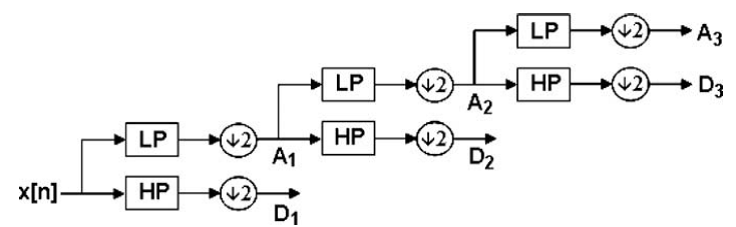
\includegraphics[width=1\textwidth]{graph.png}

\caption{Sub-band decomposition of DWT implementation}
\end{figure}
In the figure, the discrete x(n) signal crosses has the sampling rate of (100Hz) which passes iteratively through HP to generate detail coefficients (Di[n]) and crosses through LP to obtain approximation
coefficients (Ai[n]). In analysis of EEG signals, the number of levels of decomposition is chosen based on the sampling rate of the original signal and the range of frequency components which are desired to be extracted from the signal.Since the range of the useful frequency information of  EEG signals falls between $0–60$ Hz, usually decomposition level is set at 5. Selecting inappropriate number of decomposition levels causes loss of desired information.
The five level of DWT decomposition of EEG data (100 Hz) is given in Fig.2. It can be seen from Fig. 2 that the components A5 decomposition is within the delta range ($0–3$ Hz), D5 decomposition is within the theta range ($3–6$ Hz), D4 decomposition is within the alpha range ($6–12$ Hz) , D3 decomposition is within the beta range ($12-25$ Hz) and D2 decomposition is within the gamma range ($25-50$ Hz).  Therefore, in order to extract the meaningful features from the EEG signal, D2-D5 detail sub-bands and A5 approximation band are used in this study. Several successful studies related to EEG choose Daubechies wavelet as an appropriate wavelet as well as level 4 and level 5 of this function is preferred[5,6,7]. In this paper, db5 is selected as the mother wavelet for DWT decomposition. 
\begin{figure}

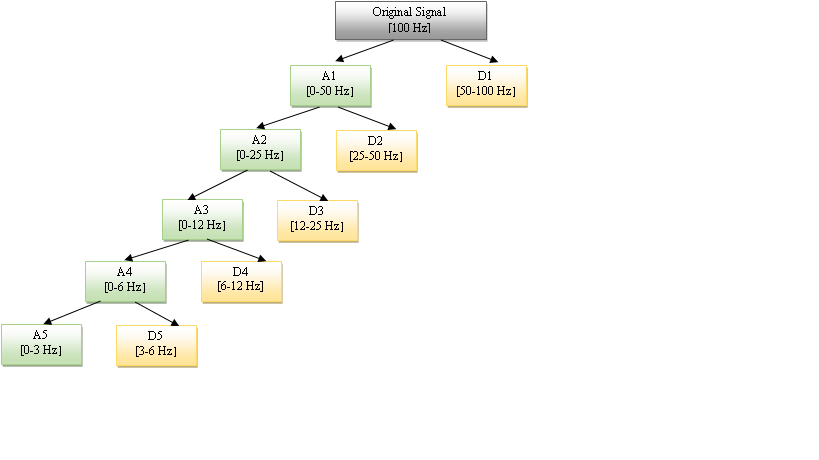
\includegraphics[width=1\textwidth]{DWT.png}

\caption{Sub-band decomposition of DWT implementation}
\end{figure}
%------------------------------------------------
\begin{figure}

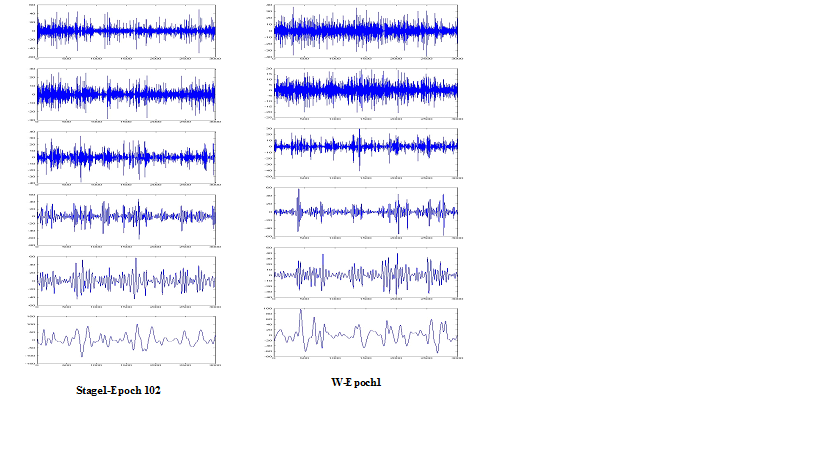
\includegraphics[width=1\textwidth]{stages.png}

\caption{Sleep Decomposition}
\end{figure}
\section*{Specifications of Dataset}

The EEG dataset is available online at PhysioBank [8]. The polysmnographic (PSG) sleep recordings included signals from EEG ( Fpz-Cz and Pz-Oz channels), horizontal EOG, submental chin EMG and an event marker. Well-trained technicians scored manually hypnograms based on the 1968 Rechtschaffen and Kales manual [9].
There are two subsets of data. In the first set, 20 healthy subjects were selected in order to study the effects of age on sleep. Two EEG datasets (about 20 hours) were recorded during two subsequent day-night periods for each subject at their home. In the second dataset, 22 subjects that had difficulty in falling sleep were selected from a study of Temazepam effects on sleep. The PSGs (about 9 hours) were recorded in the hospital during two nights.




%------------------------------------------------

\section*{Conclusion}


\begin{enumerate}
\item 
\item 
\end{enumerate}



%----------------------------------------------------------------------------------------
%	BIBLIOGRAPHY
%----------------------------------------------------------------------------------------

\bibliographystyle{unsrt}

\bibliography{sample}

%----------------------------------------------------------------------------------------

\end{document}